


\begin{firstonly}
\chapter{Getting started}
\label{cha:getting-started}
\minitoc
\notesurl{intro0}

\section{Welcome}


  Hello and welcome. In this first, introductory, lab we're going to
cover some of the basic things you'll need to know about the IT
infrastructure here in the School of Computer Science, and get your
Raspberry Pi set up so that you can get going quickly in the next lab.
Some of what we tell you may well seem very obvious to you, and if
that's the case we ask you to be patient. Some other things might
not be so obvious...

\end{firstonly}


\begin{pgtonly}
  
\section{Computing Infrastructure}
\label{cha:getting-started}
  Hello and welcome. In this introductory lab we're going to
cover some of the basic things you'll need to know about the IT
infrastructure here in the School of Computer Science.
Some of what we tell you may well seem very obvious to you, and if
that's the case we ask you to be patient. Some other things might
not be so obvious...

These notes are a modified version of some that we use in our first year Undergraduate programme. We have tailored them for PGT students, but there may be some places where they betray their origins.
\end{pgtonly}

In this and every lab there will be staff, consisting of academic staff and postgraduate students, around to help you. If you're stuck or find something that you really can't understand, then \emph{please ask for help}; that's what the lab staff are here for, don't just sit there getting frustrated. The postgraduate students are known as \concept{Teaching Assistants}, or \concept{TAs} for short, although up to 2014 they were referred to as \concept{Demonstrators}. We will try to use the new name, but inevitably both will be used for a while.


\section{About these notes}
\subsection{Breakout boxes}

Scattered throughout the main text of these exercises there are information boxes of various kinds:
\\

\begin{tabular}{m{1.5cm}m{12cm}}
{\includegraphics[width=1.5cm]{images/bomb}} & \textbf{Danger!} The bomb icon explains problems and pitfalls, and how to avoid them. It's really important that you read these sections, or you may regret it later.\\
  \\

\begin{firstonly}
    
\includegraphics[width=1.5cm]{images/rpi-logo} & \textbf{Raspberry Pi Facts and Factoids.} These sections explain useful but non-essential things about the Raspberry Pi. If you're pushed for time, you can safely skip these boxes and perhaps come back to them another time.\\
\\

\end{firstonly}

  \includegraphics[width=1.5cm]{images/diversion} & \textbf{We digress\ldots} Boxes marked with this icon contain digressions and facts that are hopefully interesting but are probably tangential to the main flow of the exercise.\\
\includegraphics[width=1.5cm]{images/roadblock} & \textbf{Stop here\ldots} Boxes marked with this icon contain checkpoint activities that you should complete before proceeding further.\\
\end{tabular}

\subsection{Styles and conventions}

We'll be using various typographic styles to indicate different things throughout these notes. When we introduce new concepts, or use terms that have a different meaning in computer science to their everyday use, they will appear \concept{like this}, and will be explained in the nearby text. Things that are either the input or output to commands will appear \ttout{in this font}. And many words or phrases will have a little `w' after them, meaning that if you click on the term (if you're reading the notes online) or type the phrase into \wikipedia{wikipedia}{Wikipedia} (if you're reading this on paper), you should be taken to a sensible definition in case you want to learn more about something that we've touched on here.

Where you see text in square brackets [LIKE THIS] it will mean that when you're typing things you should replace the text with something that the text describes; for example [NAME OF THIS CITY], would become Manchester.

\section{The CS labs setup}

All the desktop PCs in the labs in the Kilburn building are
`dual-boot': they can be started up running either Linux or
Windows. This is for flexibility -- the labs for most course units  use
Linux, but some use Windows, and of course, outside the labs, you're free to use
whichever you prefer for any aspect of your studies that does not require use of a particular operating system. If you're not
familiar with Linux, don't worry. We'll be telling you a bit about it
in this lab, and you'll be looking at it in much more detail in subsequent labs.

\section{Using Windows}
\label{sec:using-windows}

We'll start with Windows, so the first thing we need to do is to make
sure your PC is running Windows. Have a look. If it is, and the screen
looks like Figure~\ref{figure:welc-screen}, then you will not need to
reboot, but please read the next bit anyway, because at some point you
may need to reboot from Linux to Windows.

If your PC is currently in Linux, showing a black screen with a login prompt,  you need to reboot the PC. To do
this, press \ttout{ctrl}, \ttout{alt} and \ttout{delete}.

This will probably cause strange messages to appear on the screen,
disappear, and be replaced by yet more strange messages. Now look at Figure~\ref{figure:welc-grub}: when you see something like that on the screen press \ttout{space} you will need to respond. Meanwhile, be patient,
watch it all happen, and don't worry what it all means.

After a while,
everything should settle down and the screen will look like
Figure~\ref{figure:welc-grub}; press \ttout{space} now!

\begin{figure}
\centerline{\includegraphics[width=15cm]{images/TH-win-welcome}}
\caption{The Windows7 Welcome screen.}
\label{figure:welc-screen}
\end{figure}

\begin{figure}
\centerline{\includegraphics[width=15cm]{images/TH-grub-win}}
\caption{The boot selection menu screen.}
\label{figure:welc-grub}
\end{figure}

This is where you decide whether to start up Windows or Linux. \emph{If you do nothing when this screen appears, the computer automatically boots into the default operating system after a fixed timeout period. By pressing the space bar (any other key would have done) you have stopped this timeout process. }

Now use the
up/down arrow keys on the keyboard to highlight the line
reading \ttout{Windows 7}, and press the \ttout{enter} key. After a short while, the Windows 7
welcome screen will appear, as shown in Figure~\ref{figure:welc-screen}. Now use  \ttout{ctrl-alt-del} again as instructed and you should see the Windows 7 login screen, as shown in Figure~\ref{figure:login-screen}.

\begin{figure}
\centerline{\includegraphics[width=15cm]{images/TH-win-login}}
\caption{The Windows 7 login screen.}
\label{figure:login-screen}
\end{figure}

To log in to your personal account, type in your username (this is an
8-character name usually starting with an `m' that you were given at registration). Your password will
be the one  you set at registration. If your password doesn't work, or if you've forgotten it,
you need to fix this urgently. You can login on a machine running Windows,  with the username \ttout{register} and password \ttout{register}, then follow the instructions.

If you forget your password later on, you can also use one of the following methods:
\begin{itemize}
\item If you have access to a web browser, use the password recovery page at\\ \url{https://iam.manchester.ac.uk/recover}
%\item Visit the \verb|it.changes| Helpdesk in Kilburn Lower First area (Welcome Week, 09:00 -- 17:00)
\item You can also contact the University IT helpdesk (opening hours are Monday to Friday 9am to 5pm) by phone on 0161 306 5544, or dial 65544 from a University internal phone; or you can visit a helpdesk either on the ground floor of the Kilburn Building, in the Main Library (Building 55 on
the Campus Map), or in the Alan Gilbert Learning Commons (building 63).
\item Remember, if you need help, ask!
\end{itemize}

Once you're logged in, go to your My Manchester page in a web browser, at

\url{https://my.manchester.ac.uk}

You will have to authenticate again to access this page, which should look something like Figure~\ref{figure:welc-mymanchester}.

% \begin{demonote}
% Does it still look like this? Could the arrow be made a bit clearer?
% \end{demonote}

\section{Reading your email}

We use email extensively in the School, so it's vitally important that
you read your mail regularly---we work on the assumption that you'll be checking your School email at least once a day (and probably much
more often). On the My Manchester page, follow the mail link (indicated by the hand drawn arrow  in
Figure~\ref{figure:welc-mymanchester}) to access your email on the
University's Office365 system. This is a system that
gives you 25GB of email storage space and an integrated calendar. You should
see a page looking something like Figure~\ref{figure:welc-mail365}.

\begin{firstonly}
Have a look around for a few minutes and check what mail you've
got. In particular, look for one with `The Monday Mail' in the
Subject line. This is an important mail you'll receive every Monday
(hence the name) throughout your 3 or 4 years with us in the
School which  tells you what's going on each week. Take a moment to read it now. You can always read the Monday Mail, by the way, at the archive located at\\  \urlnop{studentnet.cs.manchester.ac.uk/ugt/mondaymail/}
  
\end{firstonly}

\begin{figure}
\centerline{\includegraphics[width=15cm]{images/mymanchester.pdf}}
\caption{Your MyManchester page.}
\label{figure:welc-mymanchester}
\end{figure}

\begin{figure}
\centerline{\includegraphics[width=15cm]{images/outlook.pdf}}
\caption{Your Office365 email.}
\label{figure:welc-mail365}
\end{figure}

\label{sec:reading-your-mail}

Office365, like most modern email systems, supports the IMAP
protocol -- which means that you can access your mail from any device
that can run an IMAP mail client. Some examples of such clients are:
Mozilla Thunderbird, Mac Mail, Windows Live Mail and mail apps on mobile devices. No matter what
client you use, you need to tell it the appropriate settings. The mechanism for finding these setting can be found in our CS student IT wiki, which is located on the web at \urlnop{wiki.cs.manchester.ac.uk/index.php/StudentFAQ/IT}. Look for the answer to the question 'How do I configure my favourite IMAP mail client?'. This wiki provides help about the IT infrastructure within the School; it is one of several School FAQ lists, which can be found at \urlnop{wiki.cs.manchester.ac.uk/index.php/StudentFAQ}. Please make use of these valuable sources of information.

Once you've found the settings, use Office365 to email this information to yourself, to your
University account, which is usually of the form:

\url{firstname.lastname@student.manchester.ac.uk}

You should also write this information down somewhere you can find it, as you will need it \firstorpgt{in a later lab}{later}  when you may not have access to your email.

\enlargethispage{\baselineskip}
\emph{You'll need this information later so please don't delete this email after you've read it.}


Finally, if you use an IMAP mail client on your phone or mobile
device, you can configure it to use the settings you've just found, and check
that you can read and send email successfully. It's probably best to try this later as the mobile signal in the lab is not good.

That's all on Windows for now, but of course  you're free to boot an available PC into Windows  and use it at any time unless you are in a lab that requires the use of Linux.

\section{Rebooting into Linux}
\label{sec:rebooting-into-linux}

So let's reboot the PC, and start it up in Linux. First, log out of
Windows by selecting the Windows icon in the bottom left of the screen and then \ttout{Log off}. Get back to the login screen, click the
small icon in the lower right of the screen (see Figure~\ref{figure:welc-restart}) and select \ttout{Restart}.

\begin{figure}
\centerline{\includegraphics[width=0.4\textwidth]{images/TH-shutdown-win}}
\caption{Restarting the PC.}
\label{figure:welc-restart}
\end{figure}

The system will shut down and after a while we'll be back to the boot selection menu
screen we saw earlier in Figure~\ref{figure:welc-grub}. This time, press space immediately, then use
the up/down arrow keys to select \ttout{EPS Linux (Scientific
  Linux)}. Linux will now start, and after a short while you should
see a black screen, with a white login prompt.

\pgtcommand{\endinput}
We won't login to Linux
at this stage, that can wait until a later lab, next week. We would,
however, like you to read the rest of this document, which gives you
some useful and interesting background information about Linux. If you
don't have time to finish reading it in the lab, please make sure you
do so before the next lab session.

Before we move on to this reading we would like you to make a start in setting up your very own Raspberry Pi computer. During this process there will be a period where you have to sit and wait for something to happen; this will give you a good opportunity to read the background information about Linux.
%\section{Using the School Linux system}

\section{Getting started with Raspberry Pi}

You should by now have received a bag containing all the bits you'll need to assemble your Raspberry Pi. The Raspberry Pi is an astonishing piece of hardware. Not because it is super-fast or super-powerful---it's actually quite a slow computer by today's standards---but because it is small, cheap and needs very little energy to run. Its cheapness means you can experiment with it safe in the knowledge that if you mess it up, lose it, or drop it into the canal, getting hold of a replacement isn't going to cost you much more than a text-book or a night out at the cinema. Its small size and fairly modest power requirements mean that it can be put to use in lots of applications where a regular-sized PC would be impractical.  We hope this will encourage you to experiment and explore, and to take risks playing with both its hardware and software that you might be reluctant to do on your own computer or tablet, or simply can't do with the School's lab machines.

In this lab session we start the process of setting up the  Raspberry Pi and continue in the next one to use it and get you familiar with the Pi, and with some of the basics of the Linux operating system it uses. We're going to be covering a lot of ground quite quickly, and it's important that you read these notes carefully and follow the instructions precisely for now. As the lab sessions progress, the instructions will become much less prescriptive, and we'll be encouraging you to experiment and explore much more, and to find out things for yourself. But for now, just follow our lead.

The most remarkable thing about the Pi is that, although it's not the most powerful of computers, it is capable of running the same full \wikipedia{Linux}{Linux} operating system as the machines that you'll be using in the labs for the duration of your studies, and which you'll undoubtedly encounter in your future careers. We're actually going to be using slightly different flavours of Linux on the Pi and the lab machines, but the differences are fairly minor---more on that later. Let's get started.

The Raspberry Pi itself is just the circuit board shown from the top in Figure \ref{figure:bare-rpi}. Your kit contains a Pi together with a case, SD card and power supply. If you want to replace the case with one in a different style you're welcome to do so (there are plenty available to buy online, and lots of people have made their own unique ones just for the fun of it). The Pi is reasonably robust, and you can use it without a case, but obviously it's a bit more vulnerable if it's not in a box of some sort. Figure \ref{figure:bare-rpi-underside} shows the Pi's circuit board from beneath, indicating where the micro SD card gets inserted.

\begin{rpi}{Why is it called a Pi?}
  The Raspberry Pi apparently got its name because (a) lots of other computer systems have been named after fruit (you'll know of Apple and Blackberry, but in the past there has also been at least Apricot and Tangerine), and (b) the \wikipedia{Python_(programming_language)}{Python language} was one of the first things ported to run on it. The logo was created by Paul Beech, and is based on \wikipedia{Buckminsterfullerene}{Buckminsterfullerene}, a spherical fullerene molecule more commonly called a Buckyball. Its designer pointed out that a full buckyball has 32 faces, but that only 11 are visible in the 2D logo; and that the Raspberry Pi has a 32-bit processor and an ARM11 on board.

The ARM processor, on which the Pi and the vast majority of the world's other mobile devices are based, was originally designed by a team led by \wikipedia{Steve_Furber}{Steve Furber}, who is a Professor in this School.
\end{rpi}

\subsection{Connecting the Pi}
\label{sec:connecting-pi}


\begin{figure}
\centerline{\includegraphics[width=15cm]{images/rpi2-front}}
\caption{An uncased Raspberry Pi 2. The numbered connectors are \protect\circled{1} HDMI output,  \protect\circled{2} four USB ports,  \protect\circled{4} micro-USB power input,  \protect\circled{6} stereo audio out,  \protect\circled{7} General Purpose Input/Output (GPIO),  \protect\circled{8} Ethernet.}\label{figure:bare-rpi}
\end{figure}

\begin{figure}
\centerline{\includegraphics[width=15cm]{images/rpi2-back}}
\caption{A naked Raspberry Pi from below. The ports are numbered as in Figure~\ref{figure:bare-rpi}, and in addition \protect\circled{3} shows the location of the micro SD (Secure Digital) memory card and the correct orientation of the card to insert into the Pi.}\label{figure:bare-rpi-underside}
\end{figure}

It's important that you connect the Pi up in exactly the order specified here---so even if you are familiar with using a Pi, please don't jump ahead and plug everything in at once (no harm will come to the Pi if you do, but this exercise relies on your following our instructions closely). Refer to Figure \ref{figure:cables}, and then connect your Pi up like this:

\begin{figure}
\centerline{\includegraphics[width=13cm]{images/cables}}
\caption{The following cables are available to connect up your Pi. \protect\circled{1} HDMI, \protect\circled{2} Keyboard and Mouse, \protect\circled{3} 5 Volt Micro USB power supply, and \protect\circled{4} network.}\label{figure:cables}
\end{figure}


\begin{itemize}
\item The monitors in the LF31 Lab are all fitted with an extra video lead for connecting up the Pis. We try to standardise on blue cables for connecting to a Pi. Locate the HDMI lead (labelled \protect\circled{1} in Figure \ref{figure:cables}), and plug this into the socket marked \circled{1} on Figure~\ref{figure:bare-rpi}.
\item Next we'll need to connect a keyboard and mouse. Separate the male and female USB connectors marked \protect\circled{2} on Figure \ref{figure:cables}, and plug the male end into one of the two USB sockets on your Pi (marked with \protect\circled{2} on the Figure~\ref{figure:bare-rpi}). It doesn't matter which USB socket you choose, but please make sure to reconnect this to the PC when you're done with these experiments as a courtesy to the next user.
\item \textbf{Do not connect the power or network connectors at this stage!}
\end{itemize}

Next, we need to insert the memory card that contains the Pi's operating system, and on which you'll be storing your own files (note although this is a `memory card', for the Raspberry Pi it's behaving like the `hard disk' of a regular computer, not like the \textit{memory} of a regular computer). The card you've been given comes in a little caddy that allows it to be used as a full-sized Secure Digital card, but for the Raspberry Pi Model 2 we just need the little mico SD card it contains. Carefully pop that out of the caddy and then refer to Figure ~\ref{figure:bare-rpi-underside} to see where it goes on the Pi's board. It should slide both in and out smoothly. Don't force the card in or you might damage it or the Pi -- if you're not sure, get some help.





Now you're ready to power up the Pi. In our lab setup in LF31 the power to the Pi is supplied via the monitor, so it is important that the monitor is not in standby mode. Standby is indicated by an orange light on the on/off button at the bottom right of the screen, rather than blue if it is on. If the light is orange, press it to turn the monitor off, then again to switch it back on and turn it blue. Now locate the 5v Micro USB cable (the same connector that you'll find on many modern smartphones and tablet devices); this is labelled \protect\circled{3} on Figure~\ref{figure:cables}. This goes into the socket marked \circled{3} on Figure \ref{figure:bare-rpi}. There is no power switch on the Pi, so as soon as the power cable goes in, it will start to boot (this strange term is explained in breakout box~\ref{bootbox}): the red PWR LED should light up and stay on, and you'll also notice that the OK LED (which indicates SD-card activity) to its left also flickers. If any of the other three LEDs marked FDX, LNK, or 10M are lit, then that means you've already plugged a network cable into your Pi, in which case please unplug that now!



% Moved this Danger Box to intro1
%\begin{danger}{Pi Power}
%Like most other computers, the Pi doesn't like having its power removed without being shut down properly. Although you might get away with it, there's a reasonable chance of messing up the operating system if you remove the power while the Pi is in the middle of doing something. And because the Pi runs a multi-tasking operating system, it's almost always `doing something', so pulling the power out unexpectedly is always a bad idea. You're unlikely to damage the Pi's hardware like this, but you may find that you lose work, and may have to reinstall the operating system. For instructions on how to shut the Pi down safely, see Section \ref{section:shutdown}.
%\end{danger}

Now we need to switch the input on the monitor from DisplayPort (which
is the input used by the PC under the desk) to DVI (the cable you've
connected your Pi to is a HDMI to DVI cable). On the lower-right side
of the monitor you will see 4 buttons -- see
Figure~\ref{figure:monitorswitch}. Press any of them to bring up the
monitor's menu. Now press the 3rd button down and navigate to the
input selection menu. Switch the Input to DVI and all being well you
should see a black screen containing the Raspberry Pi logo at the top
left, and white text that scrolls up the screen as the Pi boots.

\begin{figure}
\centerline{\includegraphics[width=12cm]{images/DellInputMenu.jpg}}
\caption{The Input Selection menu on the monitor. This image  of the Dell U2412M Monitor has been reproduced with the kind permission of Dell. All rights reserved.}\label{figure:monitorswitch}
\end{figure}

%When the boot process finishes for the first time (it will take somewhere
%about 20--30 seconds), if all has gone well you should see the NOOBS (New Out Of Box)
%installation tool appear (see Figure \ref{figure:noobs-install-screen}).

%\begin{figure}
%\centerline{\includegraphics[width=13cm]{images/noobs-install-screen}}
%\caption{NOOBS Install Screen}\label{figure:noobs-install-screen}
%\end{figure}

%\subsection{Installing Raspbian}

%The SD card that comes with your Pi is set up so that when you first start the device you can choose to install one of a variety of different operating systems that are compatible with the Raspberry Pi hardware. We are going to use Raspbian for all of the labs, so scroll down the list until you see an option labelled Raspbian with an SD card icon to the right, and check the left hand box as shown in Figure \ref{figure:noobs-select-raspbian}. \emph{Take care not to select the other Raspbian option with a network connection icon, as this will attempt to download Raspbian over the network.}

%\begin{figure}
%\centerline{\includegraphics[width=13cm]{images/noobs-select-raspbian}}
%\caption{Selecting Raspbian}\label{figure:noobs-select-raspbian}
%\end{figure}

%Click the Install button and you will see a final warning message as in Figure~\ref{figure:noobs-install-warning}. Click Yes to confirm, and the installation process shown in Figure \ref{figure:noobs-install-progress} will begin. This process will take around 15 minutes to complete, so while you're waiting for Figure~\ref{figure:raspi-config} to appear please use the time to read Section~\ref{sec:unix-linux} in the separate handout then come back here to complete the installation process.
%\label{page:raspbian-install}

%\begin{figure}
%\centerline{\includegraphics[width=13cm]{images/noobs-install-warning}}
%\caption{Final warning/confirmation from NOOBS}\label{figure:noobs-install-warning}
%\end{figure}

%\begin{figure}
%\centerline{\includegraphics{images/noobs-install-progress}}
%\caption{NOOBS installation progress}\label{figure:noobs-install-progress}
%\end{figure}

\begin{rpi}{Raspbian}
  Raspbian is a version of the Debian release of Linux, tuned for the Pi. If you manage to corrupt the operating system, or just want to start from scratch, then re-writing the SD card with a fresh image is reasonably straightforward: simply reboot your Pi and press the Shift key when the initial splash screen loads (you will need to be quick, as it only appears for a few seconds). This will present you with a list of options. Ensure that Raspbian is selected and then click the Install icon to re-write the SD card with a fresh image. This will erase all of the data on the Pi, so it's crucial that you make sure that you have a backup of anything important.

  If you buy a new SD card, instructions on how to get hold of the files you'll need, and how to write them to the SD card on various operating systems are available at \urlnop{www.raspberrypi.org/downloads}. You might want to think about getting a larger SD card in any case; the one we've given you is fine for the labwork we've set, but probably a bit on the small side for anything else. SD cards are widely available in shops and online, and aren't expensive. But you should check whether the specific card you're going to buy is compatible with the Pi before parting with any money---differences in the read/write speeds of some cards mean they don't play nicely with the Pi.
\end{rpi}


\begin{diversion}{Booting}
\label{bootbox}
The phrase `booting' to refer to the process of starting up some computer system has become quite commonplace, but its origins are rather strange. It's thought to have first been used in early 19th Century America as a way of describing an obviously impossible action such as to ``pull oneself over a fence by one's bootstraps''. These days it is used to refer to any self-sustaining process that is able to happen without external help.

So why is starting a computer a bootstrapping process? In order for you as a user to be able to run a program, the computer needs an operating system. But in order to load its operating system, it needs some instructions that tell it how to understand the file system. And in order to load the instructions that tell it how to understand the file system it needs to\ldots well, you get the idea. In reality, most computers have a very small set of instructions hardwired into them that begin the process of loading a  slightly more complex `bootloader', which then begins the process of loading the OS kernel and any modules needed to interact with the hardware, and then starts loading services and features of increasing sophistication that rely on the simpler ones loaded previously to function.

As an aside, you may want to consider this: if you need a text editor to write programs, how did the first text editor (which is itself a program) get written?
\end{diversion}

% At this stage you could tweak various other options that affect the
% display and the layout of keyboard being used; but conveniently the
% defaults set on the Pi will do just fine for now (it is a mostly
% British invention after all, so it defaults to UK keyboard layout!)
% Use the Tab key to move the red highlight to \ttout{<Finish>}, and hit
% Enter again;.
% Confirm that the Pi should reboot (an example of what
% this looks like is shown in Figure \ref{figure:piboot}) and this time
% when the process finishes you'll be presented by a Unix login prompt
% which will say something like:

%\begin{figure}
%\centerline{\includegraphics[width=15cm]{images/bootscreen}}
%\caption{A sample Raspberry Pi bootscreen. The exact layout and details may vary depending on the size/shape of the screen and the configuration of the Pi.}\label{figure:piboot}
%\end{figure}

%\begin{ttoutenv}
%Debian GNU/Linux wheezy/sid raspberrypi tty1

%raspberrypi login:
%\end{ttoutenv}


%\subsection{Shutting down the Pi}
%\label{sec:shutting-down-pi}

%Like any other computer, its really important that you shut your Pi down properly; if you just pull the power cord out there's a chance of corrupting the filesystem. To shut the Pi down safely you first need to login using the username \ttout{pi} and the password \ttout{raspberry}. \textbf{Note that, so that anyone standing behind you cannot even see the length of your password,  the username will appear on screen as you type it, but the password will not}.
% You will then see a screen which contains a prompt looking like

% \begin{ttoutenv}
% \textbf{pi@raspberrypi ~ \$  }
% \end{ttoutenv}

The latest generation of the Pi automatically starts a graphical user
interface; as we need to be more flexible, we will issue some commands to
disable this behaviour. Once this is done your Pi will subsequently start
from a simple command line prompt.

On the screen you will see a panel of tool icons on the top
left. Click on the icon that looks like a monitor screen. This runs a
command line terminal that you can enter commands in. Don't worry at
this stage exactly what the commands mean. Type:

\begin{ttoutenv}
sudo raspi-config
\end{ttoutenv}

followed by the Return key.

\begin{figure}
\centerline{\includegraphics[width=13cm]{images/raspi-config.png}}
\caption{The Raspberry Pi config tool. The highlight bar can be moved between the different controls using the Tab key, or up and down in the menu using the arrow keys.}\label{figure:raspi-config}
\end{figure}

% Once Raspbian has finished booting, you will  
% be presented with a configuration screen as shown in Figure \ref{figure:raspi-config}. as shown in Figure \ref{figure:raspi-config}.  

You should see a configuration screen as shown in Figure
\ref{figure:raspi-config}. Use the arrow keys to select `Boot Options',
then press Tab until \verb+<Select>+ is highlighted,
then press Return. This will bring up another configuration
screen. This time use the arrow keys to select the option `Text
console, requiring user to login'. Again use Tab until
\verb+<OK>+ is highlighted, then press Return. You should now be
back at the previous configuration screen. This time use the arrow keys to select `Change User Password` and press Return.
You'll see another message, but just select \verb+<OK>+ with the Return key to get to the password entry screen.
Don't worry about the password you're typing not appearing on the screen - that's normal! 
Select \verb+<OK>+ if the password is changed successfully, and ignore this window for now.

\begin{danger}{Don't forget your password}
It is very important that you do not forget this password; there's no easy way to get back into your Pi without resetting everything.
\end{danger}

\begin{danger}{Memory Loss}
Although the Pi uses a fairly standard Unix operating system, it's probably not quite as secure as a normal desktop machine because of its small size and easily-removable storage media. Once the Pi has booted from the SD card, it's about as secure as any other Linux machine, but because the memory card is easily removable, it can trivially be connected to another machine as a `removable media' device; and at that point the host machine can almost certainly see its contents, including any of the files you've created, because the filesystem itself isn't encrypted. And because the Pi is small and portable, it's easier to lose it than a laptop or desktop machine; so, be careful!
\end{danger}


\section{Network Registration}

The Raspberry Pi network here is separated from the main network and the internet, and you will be unable to access other networks until you register your Pi.
Now that your password isn't the same as the `out of the box' Pi one, it's safe to plug your Pi into the network. Locate the blue ethernet cable poking out of the desk (labelled \protect\circled{4} on Figure~\ref{figure:cables}) on page~\pageref{figure:cables}; plug that into the appropriate socket on your Pi (number \circled{8} on Figure~\ref{figure:bare-rpi}, page~\pageref{figure:bare-rpi}).
Click the globe icon in the panel at the upper left of the screen. The web browser should appear. Type any URL into the address bar and press enter - you should be redirected to the registration page.
Simply enter the login details you use for MyManchester and click accept. If you register successfully, you should be told to shutdown your Pi. First, switch back to the command line window.

\begin{figure}
\centerline{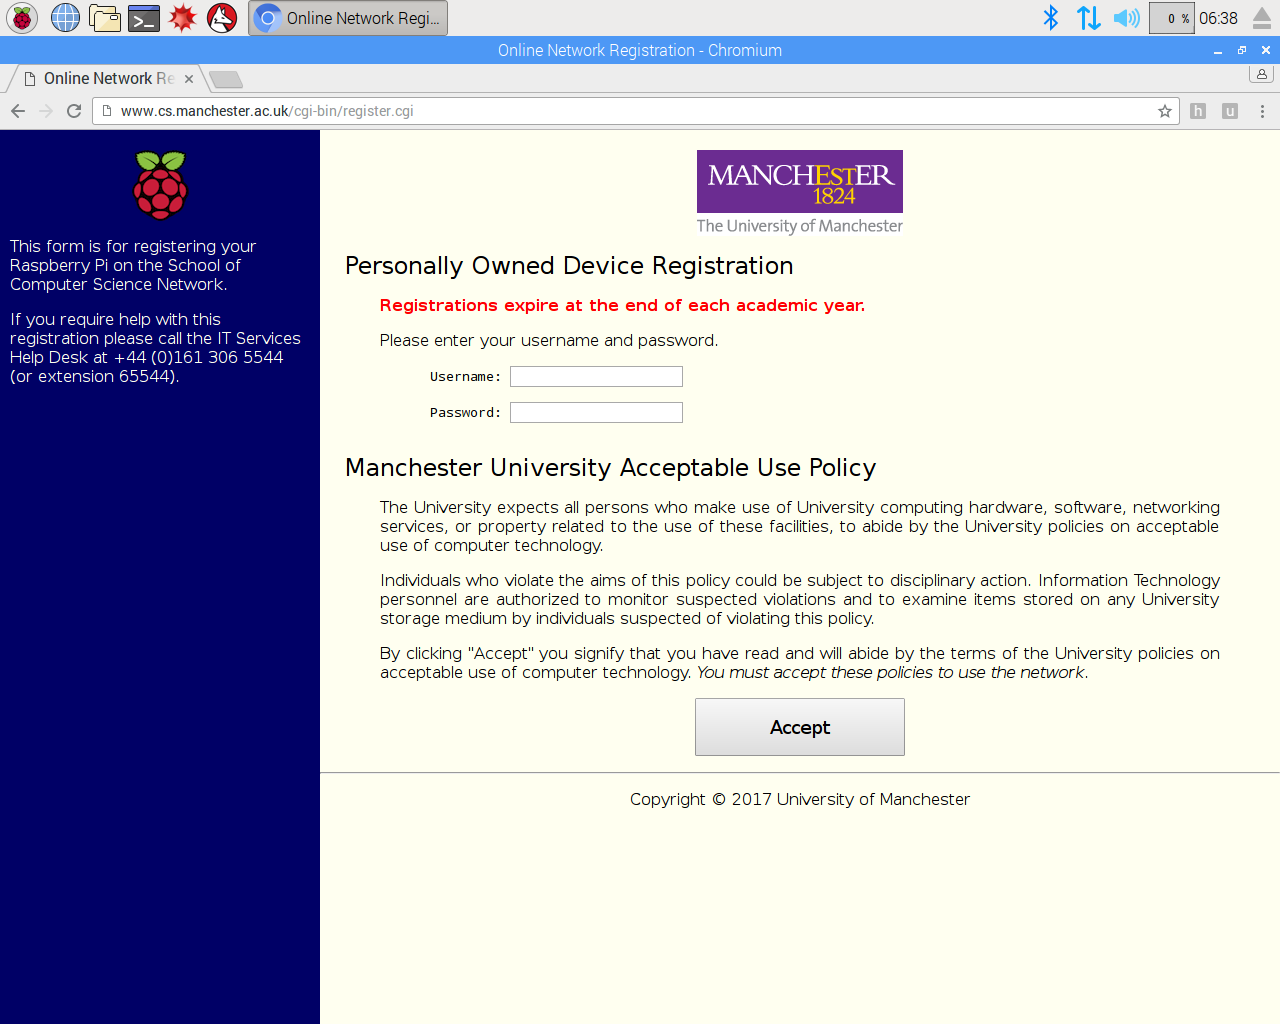
\includegraphics[width=13cm]{images/NetReg.png}}
\caption{The NetReg registration page.} \label{figure:netreg}
\end{figure}

Use the tab button to select \verb+<Finish>+ then press Return. You should now see a screen asking `Would you like to reboot?'. Tab to \verb+<No>+ then press return.

You should now be back in the command line Terminal, where you can stop the Pi by typing
%$

\begin{ttoutenv}
sudo halt
\end{ttoutenv}
followed by the Return key.

\noindent We'll explain a bit more about what's going on here in the next lab session, but for now please just follow the instructions.

%\noindent You'll see the a series of messages scroll past that look rather like those you saw during the boot process. This shouldn't be surprising, since what the operating system is doing now is shutting down all the things that it started up when you booted the machine, roughly in reverse order.

The  Pi will now power itself down; the ACT LED will go off, the screen should go black, and only the red PWD LED will remain lit on the circuit board. At this point it's safe to pull the Micro-USB cable out of the Pi. Please make sure you reconnect the USB connector for use with the PC  as a courtesy to the next user, \emph{taking care to connect the USB cable the correct way round. } Make sure that you leave the desktop PC booted into Linux.

That's all we want you to do with the Raspberry Pi for this session, we will start using it in earnest in the next session.  When you have completed the work for this session, please tell the lab supervisor so we know how you're getting on. Remember, if you don't finish it during the lab session, please try to do so before the next one.

\textbf{Please make sure you bring your Pi and this set of notes to all the introductory lab sessions.}

\cleardoublepage

\section{Unix and Linux}
\label{sec:unix-linux}


Over the next couple of weeks you will be undertaking a number of
introductory labs to familiarise yourself with the School's computing
infrastructure. Much of this is based on devices and machines running Linux, a
variant of the Unix family of operating systems; this document
provides some background on Unix and explains why we think it is
important. It would very useful if you could read this before you
attend the first introductory labs, where the emphasis will be on
leading you through a series of tasks to explore our setup.

\subsection{Operating Systems}

An \wikipedia{Operating_system}{operating system} (OS) is a suite of
software that makes computer hardware usable; it makes the `raw
computing power' of the hardware available to the user. You're
probably most familiar with
the \wikipedia{Microsoft_windows}{Microsoft Windows} and
Apple \wikipedia{OS_X}{OS X} families of operating systems for
`desktop' computers, and \wikipedia{Ios}{iOS} (Apple, again) and
Google's \wikipedia{Android_(operating_system)}{Android} for mobile
devices; but many other more specialist operating systems exist, and
you'll be studying some of these and the principles that underpin OS
design in COMP25111 in your second year. In the meantime, a potted
history of OS development will tide us over\ldots

\subsection{Unix Origins}
\label{sec:unix}

In the late 1950s, an American company
called \wikipedia{Bell_Labs}{Bell Laboratories} decided that they
needed a system to improve the way they worked with their computer
hardware (it's probably quite hard to imagine what interacting with a
computer \emph{without} an operating system might be; but it wasn't
pretty and involved manually loading and running programs one by
one). Together with the \wikipedia{General_Electric_Company}{General
Electric Company} and the \wikipedia{MIT}{Massachusetts Institute of
Technology}, they set about the design of an operating system they
called \wikipedia{Multics}{Multics}: the `Multiplexed Information and
Computing Service'. Multics was hugely innovative, and introduced many
concepts that we now take for granted in modern operating systems such
as the ability for more than one program to run `at once'; but it did
rather suffer from `design by committee', and the final system was
seen at the time as being overly complex and rather bloated (`bloated'
is all a matter of perspective of course: it's sobering to realise
though that the entire Multics operating system was only around
135Kb. Today's operating systems are something like 30,000 times this
size\ldots). In the late 1960s, a group of programmers at Bell Labs
created a cut-down, leaner and cleaner version of Multics that would
work on more modest hardware. Legend has it that this was to allow
them to play their favourite (only!) computer
game, \wikipedia{Space_Travel_(video_game)}{Space Travel}. In an early
example of the trend of giving things `punny' names, to contrast with
the more clumsy Multics, they called this new system Unix. The
so-called \wikipedia{Jargon_File}{Jargon File} is a good source of
explanations of various bits of computer slang and their obscure
origins, and is well worth a read: in part to give some background
history, but mostly as an insight into the minds of the computing
pioneers of the past!

%\begin{htmlonly}
%(See the Unix entry in the useful and amusing
%\htmladdnormallink{Jargon
%file}{http://www.new.ox.ac.uk/admin/jargon/html/entry/Unix.html}, a
%file}{http://www.cs.manchester.ac.uk/software/jargon/html/entry/Unix.html}, a
%file}{\jargonFileUnix}, a
%`collection of slang terms used by various subcultures of computer
%\htmladdnormallink{hackers}
%{http://www.cs.manchester.ac.uk/software/jargon/html/entry/hacker.html}'.)
%{\jargonFileHackers}'.)
%\end{htmlonly}

Even though Unix is now quite old, most Computer Scientists recognise that the designers of Unix got most of the fundamental concepts and
architecture right. Given how much computing has changed since the 1960s, this was an astonishing intellectual achievement. Although Microsoft's \wikipedia{Microsoft_Windows}{Windows} is by far the most common operating system on \emph{desktop} machines, the majority of the Internet, much of the world's corporate infrastructure, virtually all supercomputers, and even some mobile devices are powered by Unix-like operating systems. So, while the polished graphical user interfaces of Windows and \wikipedia{OS_X}{OS X} appear to dominate the world of computing, most of the real hard-core and leading-edge computation relies on an elegant operating system designed nearly 50 years ago (by a team of scientists who wanted to play a game).

\subsection{Modern Unix Variants}
\label{sec:modern-unix-variants}


The history of Unix is complex and convoluted, with the system being updated, re-implemented, and mimicked repeatedly over the years, primarily by commercial companies who guarded their versions jealously. Figure \ref{fig:unix-history} shows a tiny fragment of the Unix's `family tree' (the full diagram, which you can find at \urlnop{www.levenez.com/unix/unix.pdf}, is \emph{many} times the size of the portion you can see here).

\begin{figure}[h!tb]
  \begin{center}
    \includegraphics[width=13cm]{images/unix}
  \end{center}
\caption{A fragment of \'{E}ric L\'{e}v\'{e}nez's Unix History chart, reproduced with permission and showing the beginnings of Linux in amongst other versions of Unix.}
\label{fig:unix-history}
\end{figure}

Although many of the branches represent interesting innovations of one kind or another, there are perhaps two that deserve particular attention. The first of these was the decision by Apple some time around the turn of the millennium to drop their own---highly popular, but ageing---bespoke operating system (unimaginatively called \wikipedia{Mac_os_9}{Mac OS 9}) in favour of a Unix-based system (now the more familiar `OS X', where `X' is both the Roman numeral `10' and a nod in the direction of the uniX nature of the OS). Although the majority of Mac users are blissfully unaware of the fact, behind the slick front-end of OS X, sits a variant of Unix. The second, and perhaps more profound of these events was the creation in 1991 by Swedish programmer \wikipedia{Linus_torvalds}{Linus Torvalds} of a Unix-like system, the source code to which \emph{he gave away for free}\footnote{`free' here in the sense both of `freedom to reuse or adapt', and also in the sense of `without charge'.}; this became known as the \wikipedia{Linux_kernel}{Linux Kernel}. Combined with other free software created by the \wikipedia{Free_software_foundation}{Free Software Foundation}, a non-commercial version of Unix called \wikipedia{GNU/Linux}{GNU/Linux} was born (GNU here is a recursive acronym for ``GNU's not Unix'', a swipe at other commercial non-Free versions; much to the annoyance of the Free Software Foundation, GNU/Linux is almost always called just `Linux'\footnote{Linux
is pronounced ``Linn-ucks'', despite the fact the name was coined by
its creator, and his name `Linus' is pronounced
``Leen-uss''!}.)

Linux has been, and continues to be, developed cooperatively by
thousands of programmers across the world contributing their effort
largely free of charge (although many are now paid to work on Linux as part
of their job). It is amazing to think that such
a project could ever happen---and it is surely a testament to the
better side of Human Nature. But what is interesting is the
observation that these programmers are not motivated by commercial
concerns, but by the desire to make good reliable software and have it
used by lots of people. Thus, Linux is a good choice of Unix: it's
Free, it's efficient, and it's reliable, and it is now used by large corporations, governments, research labs and individuals around the world. Even Google's \wikipedia{Android_(operating_system)}{Android} platform is a Linux-based mobile OS, and the  \wikipedia{Amazon_Kindle}{Amazon Kindle} is also a Linux box behind the electronic ink of its user interface (Figure \ref{fig:kindlelinux}).

\begin{figure}[h!tb]
  \begin{center}
    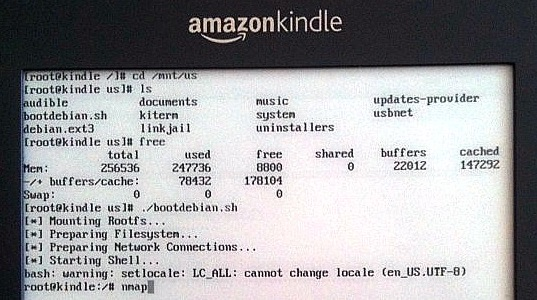
\includegraphics[width=13cm]{images/kindleroot}
  \end{center}
\caption{A photograph of Liraz Siri's `rooted' kindle, showing the Linux command prompt. Reproduced with the author's kind permission from \urlnop{www.turnkeylinux.org/blog/kindle-root}}
\label{fig:kindlelinux}
\end{figure}

One of the results of the fact that Linux is Free is that several
organisations and companies have created their own distributions of
it; these vary a bit (in fact, anybody is free to make any change they
like to Linux, and pass it on to whoever wants it). The distribution
we use in this School is \textbf{Scientific Linux}, which is
based on a distribution by a
US company called \textbf{Red Hat}.
%, which is the latest release

So, if you are to become an expert computer professional, it is
important that you understand the theory and practice of Unix based
systems. Learning Unix is not only a crucial skill for any serious
computer scientist, it is a very rewarding experience; the labs over
the next couple of weeks are designed to help you become familiar with what will be your daily working environment.

When you have completed the work for this session, please tell the lab supervisor, so we know how you're getting on.

\textbf{Please make sure you bring your Pi and this set of notes to all the introductory lab sessions.}
